\section*{Ziel}

In diesem Versuch soll mit Hilfe des Photoeffekts die maximale kinetische Energie der Elektronen in Abhängigkeit der Lichtfrequenz untersucht werden.
Dabei gilt es, wichtige Größen wie die Austrittsarbeit $W_\mathup{K}$, sowie den Quotienten $\sfrac{h}{e_0}$ mit der Elementarladung $e_0$ zu bestimmen. 
Realisiert wird dies, in dem die Abhängigkeit des auftretenden Photostroms $I$ von der verwendeten Gegenspannung $U_\mathup{G}$ gemessen wird.

\section{Theorie}
\label{sec:Theorie}

Im Laufe der Jahrhunderte entwickelte sich die Vorstellung des Lichtes und dazugehörige Theorien basierend auf durchgeführten Versuchen.
Beispielsweise ließen sich mit der Wellentheorie des Lichtes auftretende Interferenz- und Beugungserscheinungen erklären. 
Schwachstellen dieser Theorie wurden durch die Entdeckung des Photoeffekts aufgezeigt, dessen Aufbau in Abbildung \ref{fig:schematischer Aufbau}  schematisch dargestellt ist.

Betrachtet werden zwei sich im Vakuum befindliche Elektroden. 
Die Oberfläche der Photokathode ist mit einer Metalllegierung bedampft. 
Die Anode besitzt relativ zur Kathode ein positives Potential.
 Wird die Kathode mit Licht der Frequenz $\nu$ bestrahlt lässt sich über ein angeschlossenes Amperemeter ein geringer Strom $I$ messen. Dieser sogenannte Photostrom wird durch Elektronen hervorgerufen.
 Diese werden durch das Licht aus der Photokathode herausgelöst und von der Anode aufgenommen. 
 
\begin{figure}
	\centering
	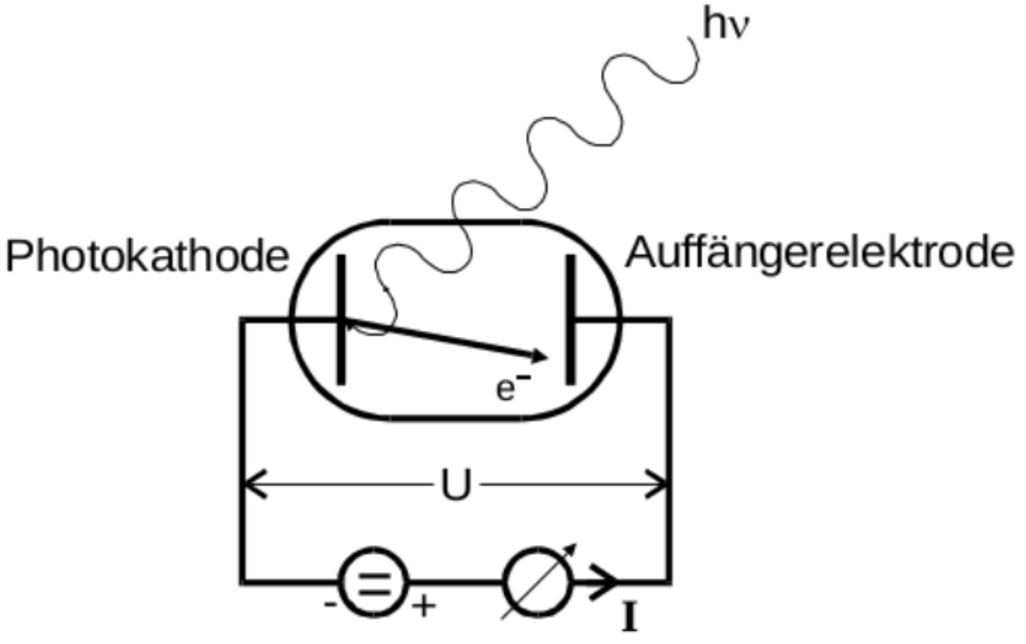
\includegraphics[width=0.8\textwidth]{Bilder/schematischer_Aufbau.pdf}
	\caption{Schematischer Aufbau der Apparatur zur Untersuchung der Photoeffekts. \cite{skript}}
	\label{fig:schematischer Aufbau}
\end{figure}
\newpage
Die wichtigen experimentellen Ergebnisse lassen sich in drei Punkten zusammenfassen.
\begin{itemize}
	\item Die kinetische Energie $E_\mathup{kin}$ der Elektronen, welche die Anode erreichen, ist unabhängig von der Lichtintensität, hängt aber stark von der Lichtfrequenz ab.
	\item Die Anzahl der herausgelösten Elektronen ist proportional zur Lichtintensität.
	\item Unterhalb einer kathodenmaterialabhängigen Grenzfrequenz $\nu_\mathup{Grenz}$ werden keine Elektronen aus der Photokathode herausgeschlagen.
\end{itemize}

Die Entdeckung des Photoeffekts ließ sich damals jedoch nicht mit der bereits vorhandenen Theorie vereinbaren.
 Grund dafür war die Annahme, dass die Energie der Strahlung gleichmäßig über die Wellenfläche verteilt ist.
Die daraufhin erdachte Korpuskulartheorie des Lichtes liefert einen Ansatz, der bis heute eine Erklärung des Effekts darstellt. Korpuskular- und Wellenmodell werden verbunden durch die Quantenelektrodynamik, welche beide Theorien als Grenzfälle mit einschließt. 
Die Korpuskulartheorie postuliert, dass die Energie des Lichtes quantisiert ist und durch Photonen -- nahezu masselose Teilchen -- transportiert wird. 
%Hier eine Frage :)
Nach \textsc{Einstein}, der 1905 die Erklärung des Photoeffekts aufstellte, sind diese Photonen gleich dem \textsc{Planck}schen Wirkungsquantum $h$. 
% Hier endet sie wieder
Mit dieser Annahme lassen sich die vorherig genannten Resultate erklären.

\begin{itemize}
	\item Die Photonen bewegen sich mit der Lichtgeschwindigkeit $c$ und tragen die Energie  $E=h\nu$.
	\item Jedes auf die Kathode treffende Photon kann höchstens ein Elektron aus der Oberfläche herauslösen. Je größer die Intensität, d.h. die Anzahl der Photonen ist, desto mehr Elektronen werden herausgelöst.
	\item Trifft ein Photon bestimmter Energie auf die Kathode, teilt sich die Energie auf in die Austrittsarbeit $W_\mathup{K}$ und die kinetische Energie $E_\mathup{kin}$ der Elektronen. $W_\mathup{K}$ muss von den Elektronen geleistet werden, um das Kathodenmaterial überhaupt verlassen zu können. Ist die Energie des Photons aufgrund einer niedrigen Frequenz zu gering, um den Elektronen das Verlassen der Anode zu ermöglichen, treffen keine Elektronen auf die Anode. Dies hat zur Folge, dass für den Photostrom $I=\SI{0}{\ampere}$ gilt.
\end{itemize}

Die kinetische Energie $E_\mathup{kin}$ der schnellsten Elektronen wird über die Gegenfeldmethode bestimmt. 
Dazu wird die Gegenspannung $U_\mathup{G}$ so lange variiert, bis der gemessene Photostrom $I$ gegen Null geht. 
Spätestens, wenn die Beziehung

\begin{equation}
	e_0 U_\mathup{G}=\frac{1}{2}mv²_\mathup{max}
\end{equation}

erfüllt ist, verschwindet der Stromfluss.
Die Energie der Elektronen setzt sich zusammen aus

\begin{equation}
	h\nu=e_0 U_\mathup{G}+W_\mathup{K}.
	\label{eq:einstein}
\end{equation}

In der Realität tritt jedoch kein unvermittelter Stromabfall bei $U = U_\mathup{G}$ auf. 
Schon für $U< U_\mathup{G}$ fällt der Strom ab.
Grund dafür ist, dass die sich in der Metalloberfläche befindlichen Elektronen nicht die gleiche Energie besitzen. 
Laut der \textsc{Fermi}--\textsc{Dirac}-Statistik erstreckt sich die Energie der Leitungs- und Valenzelektronen in Feststoffen von Null bis zur \textsc{Fermi}-Energie $\zeta$, die durchaus in der Größenordnung einiger $eV$ liegen kann.
Bei höheren Temperaturen gilt sogar $E_\mathup{e}>\zeta$. 

%Außerdem erreichen nicht alle herausgelösten Elektronen, bedingt durch die geringe Fläche der Elektroden, die Anode. 
%Besitzt das Anodenmaterial eine höhere Austrittsarbeit $W_\mathup{A}$ als die Kathode kann es vorkommen, dass kein Photostrom gemessen wird obwohl der Effekt prinzipiell möglich wäre da $h\nu>W_\mathup{K}$. 
%Die Elektronen müssten in diesem Aufbau ein gegen Gegenfeld anlaufen, da $h\nu<W_\mathup{A}$.
% Wird nun statt einer Gegenspannung $U_\mathup{G}$ über $U_\mathup{B}$ für ein beschleunigendes Potenzial gesorgt, erreichen die Elektronen die Anode wieder.
%Für eine relativ hohe Bremsspannung $U_\mathup{G}$ kann ein negativer Strom gemessen werden, welcher die Messung erschwert da der Photostrom $I$ überlagert wird.
